\subsubsection{08.01.15}

\begin{enumerate}
	\item Время начала и окончания собрания: 14:00 - 23:00
	
	\item Цели собрания: 
	\begin{enumerate}
		
	  \item Установить на механизм опрокидывания ковша один мощный сервопривод.
		
	  \item Установить ковш на сервопривод.
		
	\end{enumerate}
	
	\item Проделанная работа:
	\begin{enumerate}
		
	  \item К сервоприводу была прикреплена балка из набора Tetrix, на которой было решено прикрепить ковш.
		
	  \item Новый сервопривод был протестирован. Результат положительный: сервопривод способен опрокинуть ковш с пятью большими мячами даже когда тот прикреплен к нему за верхнюю часть. Это позволит нам установить сервопривод на самый верх направляющей подъемника, благодаря чему нам не нужно будет перед забрасыванием в любую корзину полностью раздвигать подъемник, а затем опускать его на высоту корзины, поскольку не до конца раздвинутые рейки не будут мешать опрокидыванию.
		
	 % \item Сервопривод был установлен на подъемник.
     % \begin{figure}[H]
     % 	\begin{minipage}[h]{1\linewidth}
     % 		\center{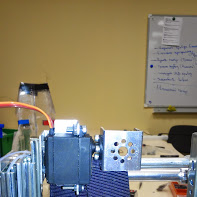
\includegraphics[scale=0.2]{days/08.01.15/images/01}}
     % 		\caption{Сервопривод с прикрепленной к нему балкой}
     % 	\end{minipage}
     % \end{figure}	
      
      \item Затем было решено присоединить балку к сервоприводу через шестеренку с передаточным отношением 1:1. Это необходимо для снятия осевой нагрузки с вала сервопривода.
      
      \item Ведущая шестеренка была зафиксирована на вал сервопривода.
      
      \item Ось с ведомой шестеренкой была закреплена с помощью двух пластин, одна из которых была прикреплена к направляющей, а вторая к креплению сервопривода.
      \begin{figure}[H]
      	\begin{minipage}[h]{0.47\linewidth}
      		\center{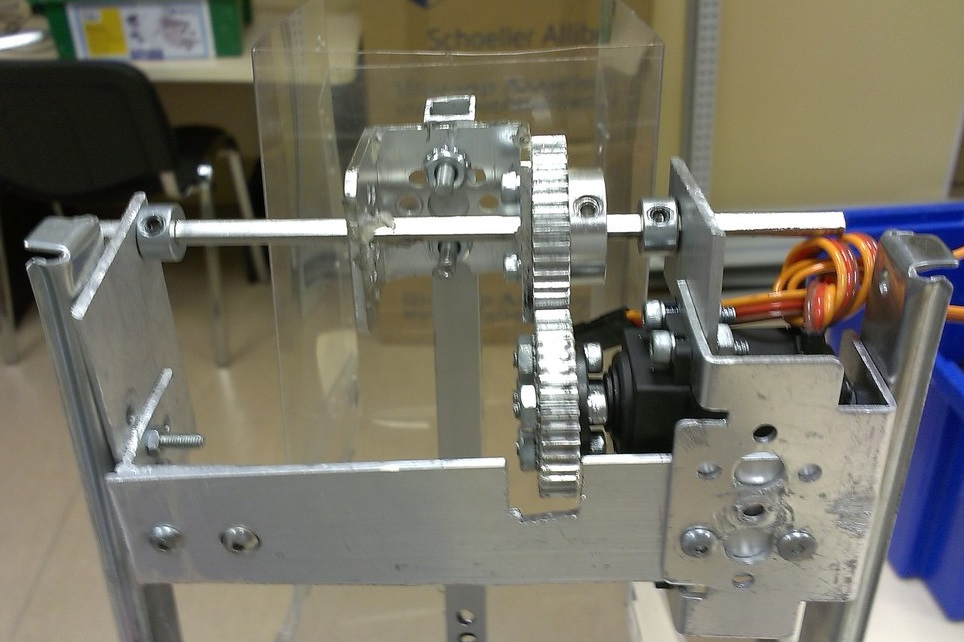
\includegraphics[scale=0.2]{days/08.01.15/images/02}}  
      	\end{minipage}
      	\hfill
      	\begin{minipage}[h]{0.47\linewidth}
      		\center{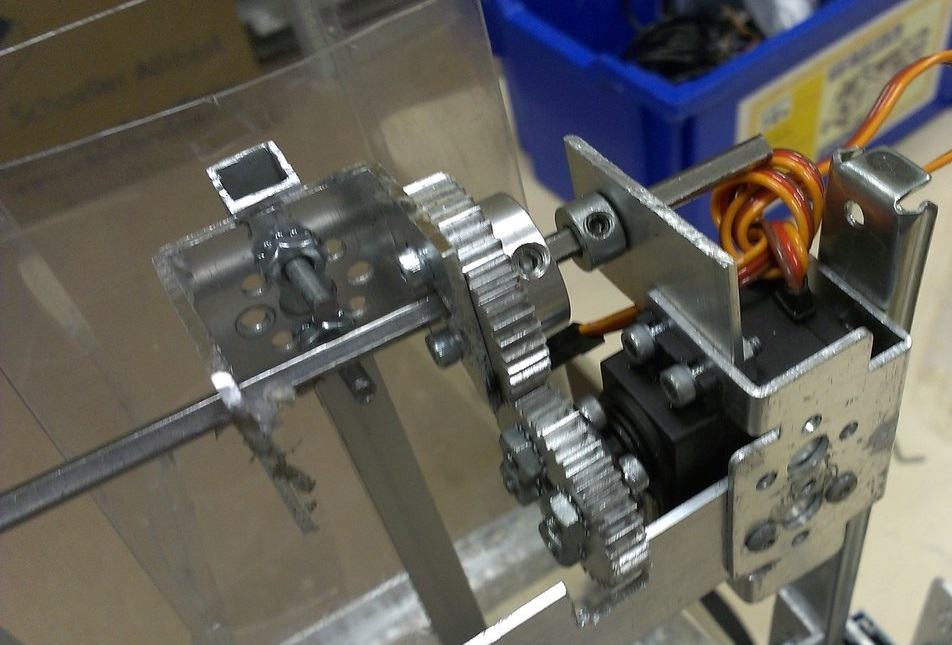
\includegraphics[scale=0.2]{days/08.01.15/images/03}}
      	\end{minipage}
      	\vfill
      	\begin{minipage}[h]{0.2\linewidth}
      		\center  
      	\end{minipage}
      	\begin{minipage}[h]{0.6\linewidth}
      		\caption{Окончательная версия механизма опрокидывания ковша (фотографии сделаны после установки ковша)}
      	\end{minipage}
      \end{figure}
      	      
      \item Было замечено, что если гайки на креплении сервопривода немного раскручиваются, то вторая пластина разбалтывается и ведомая шестеренка отходит от ведущей. Во избежании этого было решено соединить ось с ведомой шестеренкой и вал сервопривода с помощью специальной дополнительной пластины.
      
 	\end{enumerate}
 	\item Итоги собрания:
 	\begin{enumerate}
 		
 	  \item Механизм опрокидывания ковша частично завершен.
 		
 	  \item Ковш не установлен. 
 		
 	\end{enumerate}
 	\item Задачи для последующих собраний:
 	\begin{enumerate}
 		
 	  \item Изготовить и установить пластину, соединяющую вал сервопривода с осью и ведомой шестеренкой.
 		
 	  \item Закрепить ковш на сервоприводе.
 		
 	  \item Изготовить и установить провод, соединяющий сервопривод, опрокидывающий ковш, с сервоконтроллером.
 				
 	\end{enumerate}
\end{enumerate}
\fillpage